\documentclass[openany]{book}

\usepackage{amsmath}
\usepackage{listings}

\usepackage{booktabs}
\usepackage{graphicx}
\usepackage{multirow}
\usepackage{makecell}
\setcellgapes{5pt}

\usepackage[utf8]{inputenc}
\usepackage{polski}

\DeclareMathOperator*{\argmin}{arg\,min}

\title{Detekcja oszustw z wykorzystaniem metod wrażliwych na koszt}
\author{Patryk Wielopolski}

\begin{document}
	
	\newcommand{\htx}{h_{\theta}(\boldsymbol{x_i})}
	\newcommand{\es}{\mathcal{S}}
	\newcommand{\ef}{\mathcal{F}}
	\newcommand{\iks}{\boldsymbol{x}}
	\newcommand{\bes}{\boldsymbol{S}}
	\newcommand{\yht}[1]{y_i^{(#1)}}
	\newcommand{\ylab}[2]{\text{#1}_{\text{#2}}}
	
	\newenvironment{talign}
	{\align}
	{\endalign}
	
	\newenvironment{talign*}
	{\csname align*\endcsname}
	{\endalign}

\maketitle

\tableofcontents

\chapter{Wstęp}
	% TODO: Wykres potwierdzający rosnąca ilość transakcji kartami kredytowymi.
	Wraz z postępującym rozwojem technologii w ostatnich latach, który umożliwia Nam posługiwanie się kartami kredytowymi w codziennych transakcjach, podczas zakupów w internecie, a także ostatnimi czasy również i za pomocą urządzenie elektronicznych takich jak telefony komórkowe lub inteligentne zegarki, znacząco wzrosła ilość transakcji dokonywanych drogą elektroniczną. Niewątpliwie zwiększyło to wygodę dokonywania zakupów, natomiast z drugiej strony spowodowało to istotny wzrost możliwości dokonywania przestępstw wynikających z tego rodzaju płatnościami, tj. przekazania numeru karty nieznajomym, utraty lub kradzieży karty, kradzieży przesyłki lub skopiowania danych karty, które zwykle kończą się pojawieniem się na koncie nieautoryzowanych płatności.

	\begin{figure}[h]
		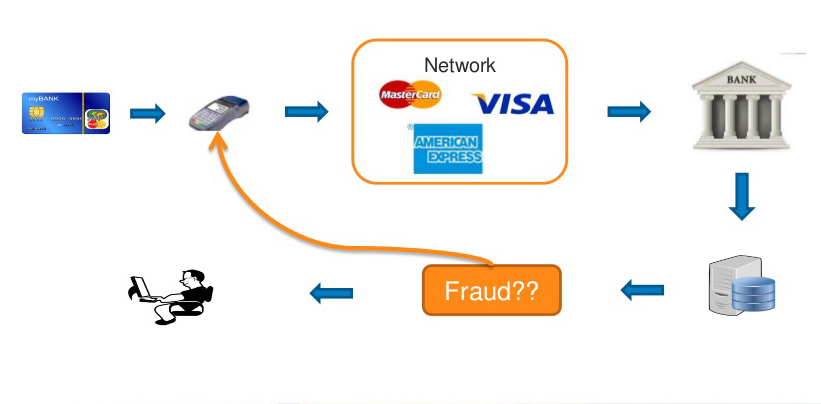
\includegraphics[width=\linewidth]{images/credit-card-flow.jpg}
		\label{credit-card-flow}
		\caption{Schemat przepływu informacji związanych z płatnością kartą kredytową. Źródło: Prezentacja A.Bahnsena podczas Konferencji Analytics 2013; https://www.slideshare.net/albahnsen/correa-bahnsen-alejandroanalytics2013slideshare}
	\end{figure}

	Banki oraz instytucje finansowe w celu przeciwdziałania takim działaniom umieszczają specjalistyczne systemy detekcji oszustw w procesie dokonywania płatności, który jest przedstawiony schematycznie na Rysunku \ref{credit-card-flow}. W momencie przyłożenia karty kredytowej do terminala następuję połączenie z operatorem karty, który następnie łączy się z bankiem klienta. Kolejno w odpowiednich bazach danych sprawdzane są dostępne środki, a także poprawność transakcji. W tym momencie działa nasz system, który w razie wykrycia niezgodności odrzuca transakcję, a sprawa jest kierowana do analityka, który bliżej przygląda się sprawie.

	Jak możemy zauważyć system do detekcji oszustw stanowi jedynie pewien element całego schematu. Do niedawna najbardziej popularnym sposobem do wykrywania oszustw były systemy oparte na regułach biznesowych. Przykładowe reguły, które mogą być używane w takich modelach mogą przyjmować następującą postać:
	\begin{itemize}
		\item Więcej niż 4 wypłaty z bankomatu w ciągu godziny;
		\item Więcej niż 2 transakcje w ciągu 5 minut;
		\item Transakcja w sklepie karta a następna zaraz w internecie.
	\end{itemize}
	W przypadku, gdy rozpatrywana transakcja spełnia chociaż jedną z reguł to jest ona blokowana i użytkownik jest informowany o odrzuceniu transakcji. To podejście jest stosunkowo łatwe do implementacji oraz jest bardzo proste do interpretacji, lecz niestety oszuści wraz z upływem czasu wpadają na nowe pomysły w jaki sposób można dokonywać oszustw, natomiast systemy złożone ze sztywnych reguł nie są w stanie wykrywać nowych zachowań i generować coraz to nowszych reguł. Tą niedogodność są w stanie rozwiązać model uczenia maszynowego, które tworzą pewnego rodzaju reguły, które nie są bezpośrednio wprowadzane przez użytkownika, lecz automatycznie wykrywane przez algorytmy na podstawie dostarczonych danych historycznych. Wraz z dynamicznym rozwojem tej dziedziny nauki zaczęły powstawać coraz bardziej wyrafinowane modele, które ostatecznie są wykorzystywane w produkcyjnych środowiskach instytucji finansowych. Niestety standardowe podejście do modelowania predykcyjnego zakłada równy koszt popełnienia błędu, co nie jest prawdą w tym jak i w wielu innych praktycznych zastosowaniach. Stąd powstała motywacja do rozwoju metod, które biorą pod uwagę tą różnicę.
	
	Wybór tematu pracy był naturalną konsekwencją codziennej pracy nad modelami predykcyjnymi wykorzystywanymi do detekcji oszustw w szkodach komunikacyjnych. Zauważony w trakcie prac problem nierównego kosztu pomyłek doprowadził mnie do poszukiwania metod, które będą adekwatne do tego rodzaju wyzwań. W ten sposób trafiłem na prace dr Alejandro Correa Bahnsena, które poruszały to zagadnienie dla modelowania ryzyka kredytowego, prognozy rezygnacji z usług przez klientów, marketingu bezpośredniego oraz detekcji oszustw w transakcjach kartami kredytowymi. Z uwagi na bliską analogię ostatniego przykładu z moim pierwotnym problemem zdecydowałem się podjąć bliższemu przyjrzeniu temu tematowi.
	
	Celem pracy jest opisanie i porównanie klasycznych oraz wrażliwych na koszty metod predykcyjnych z dziedziny statystyki oraz uczenia maszynowego w problemie detekcji oszustw na kartach płatniczych, a także przeprowadzenie eksperymentu porównującego skuteczność poszczególnych metod. Wykorzystane zostaną modele takie jak regresja logistyczna, drzewo decyzyjne, las losowy oraz algorytm XGBoost wraz z odpowiednimi modyfikacjami oraz metody optymalizacji progu oraz minimalizacji ryzyka bayesowskiego.
	
	Praca jest zorganizowana w następujący sposób: rozdział drugi jest wstępem teoretycznym, który zawiera opis miar skuteczności modeli oraz aspekt teoretyczny wykorzystanych metod. Rozdział trzeci prezentuje opis eksperymentu wraz z wynikami oraz wnioskami. Ostatnia część podsumowuje całość pracy.

\chapter{Wprowadzenie teoretyczne}

	Wprowadzenie teoretyczne zawiera wszelkie potrzebne informacje dotyczące użytych w dalszej pracy metod z dziedziny statystyki oraz uczenia maszynowego. W~szczególności zaczniemy opisania samych modeli, które dzielą się na dwie kategorie: standardowe oraz wrażliwe na koszt. Pierwsze z~nich są powszechnie znane i wykorzystywane w bardzo wielu obszarach zastosowań. Drugie z nich są specyficzne dla pewnej klasy problemów, gdzie koszt popełnienia poszczególnych błędów jest różny i dzielą się one na dwie podkategorie - \textit{Cost Sensitive Training} oraz \textit{Cost Sensitive Classification}. Dalej zostaną wprowadzone miary skuteczności modeli predykcyjnych, które będą nam potrzebne do stwierdzenia, który z otrzymanych modeli jest najlepszy.
	
	% TODO: Kilka słów o MLu w ogólności

\section{Standardowe modele}

	

\subsection{Regresja logistyczna}
\label{reg-log}
	Regresja logistyczna należy do jednego z najbardziej podstawowych modeli statystycznych używanych do problemów klasyfikacyjnych. Jest to model, w którym zakładamy, że logarytm szans jest kombinacją liniową predyktorów, co możemy zapisać jako:
	$$ \log{\frac{p}{1 - p}} = \sum_{j=1}^k \theta^{(j)}x_i^{(j)} $$
	Po nałożeniu odpowiednich przekształceń ostatecznie otrzymujemy, że estymowane prawdopodobieństwo możemy zapisać w następującej postaci
	\begin{equation}
		\hat{p} = P(y=1|\boldsymbol{x_i}) = h_{\theta}(\boldsymbol{x_i}) = g\left(\sum_{j=1}^k \theta^{(j)}x_i^{(j)} \right)
	\end{equation} 
	gdzie funkcja $g(z)$ to sigmoidalna funkcja łączącą, która jest opisana wzorem: 
	$$ g(z) = \frac{1}{(1+e^{-z})} \text{.}$$
	
	W celu znalezienia odpowiednich parametrów definiujemy standardowa funkcja straty, która przyjmuje następującą postać:
	$$ J(\theta) = \frac{1}{N} \sum_{i=1}^N J_i(\theta) \text{,}$$
	gdzie $J_i(\theta)$ często w literaturze nazywana jest entropią krzyżową i przyjmuje postać:
	\begin{equation}
	\label{c-e}
		J_i(\theta) = -y_i log(h_{\theta}(\boldsymbol{x_i})) - (1-y_i) log(1 - h_{\theta}(\boldsymbol{x_i}))
	\end{equation}
	Następnie wykorzystując algorytm optymalizacyjny, który będzie w stanie znaleźć minimum funkcji straty, znajdujemy odpowiednie parametry modelu.
	
	\begin{figure}[h]
		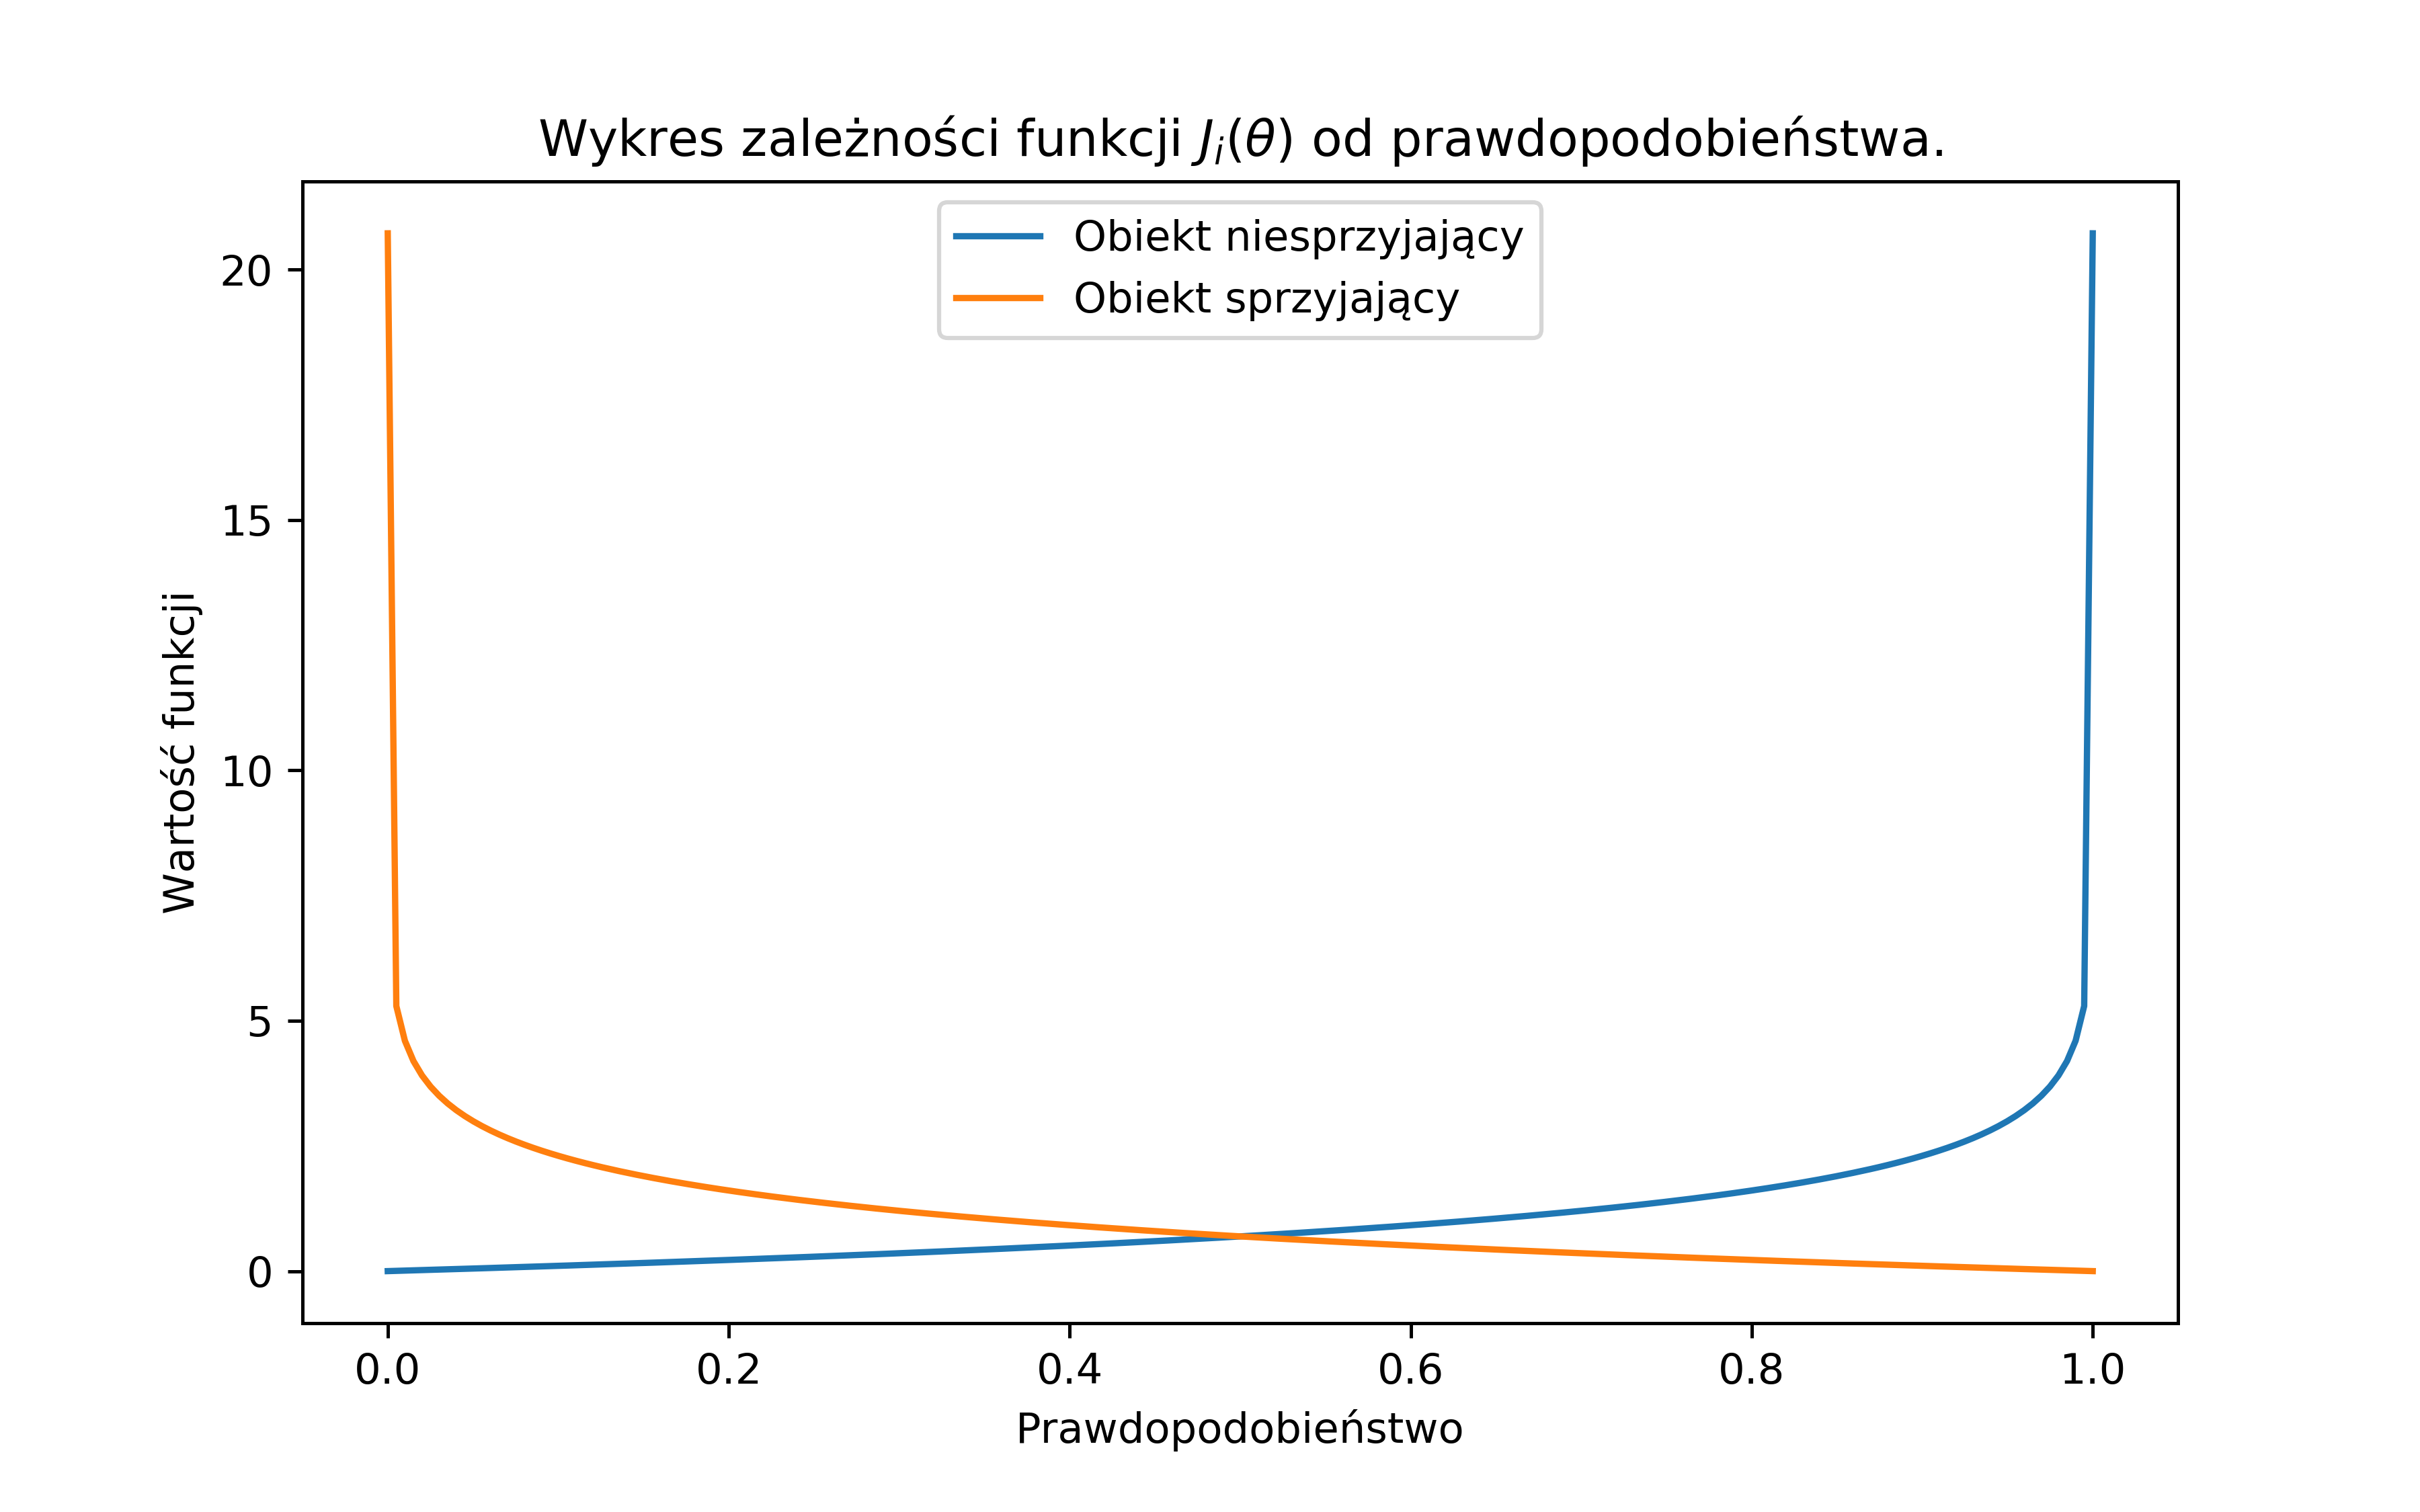
\includegraphics[width=\linewidth]{images/cross_entropy.png}
		\label{cross-entropy-plot}
		\caption{Wykres zależności funkcji entropii krzyżowej od prawdopodobieństwa predykcji danej obserwacji. Kolor niebieski przedstawia wykres dla próbki o prawdziwej klasie pozytywnej, natomiast kolor pomarańczowy dla negatywnej.}
	\end{figure}
	
    Korzystając z Rysunku \ref{cross-entropy-plot} możemy zauważyć, że koszt klasyfikacji przyjmuje następujące wartości:
	$$
	J_i(\theta) \approx \left\{
	\begin{array}{rl}
	0, &\mbox{if $y_i \approx \htx$}, \\
	\infty, &\mbox{if $y_i \approx (1 - \htx)$}.
	\end{array}{}
	\right.
	$$
	To znaczy, że w przypadku prawidłowego zaklasyfikowania danej obserwacji funkcja kosztu przyjmuje wartość bliską zeru, natomiast w przypadku pomyłki nieskończoności. Zatem stąd możemy wywnioskować, że koszty popełnienia bądź niepopełnienia błędu są następujące:
	$$ C_{TP_i} = C_{TN_i} \approx 0 $$
	$$ C_{FP_i} = C_{FN_i} \approx \infty $$
	Porównując otrzymane rezultaty z macierzą kosztów możemy zauważyć, że te wartości znacząco odbiegają od tego co w rzeczywistości chcemy otrzymać. Stąd powstaje motywacja, aby zmodyfikować podaną funkcję celu i stworzyć regresję logistyczną wrażliwą na koszt, która będzie optymalizować właściwe dla Nas wartości.
	
\subsection{Drzewo decyzyjne}
\label{drzewo}

	Drzewo klasyfikacyjne to przykład jednego z rodzaju drzew decyzyjnych, którego celem jest znalezienie najlepszego rozróżnienia pomiędzy klasami. W ogólności drzewo decyzyjne składa się z zestawu reguł.
	
	Drzewo składa się z węzłów, które są reprezentowane przez parę $(\iks^j, l^j)$, która oznacza podział zbioru obserwacji $\es$ na dwa zbiory: $\es^{l}$ oraz $\es^{r}$ względem wektora obserwacji $\iks$ oraz progu decyzyjnego $l^j$ w następujący sposób:
	$$ \es^l = \{ \iks^* : \iks^* \in \es \land x^j_i \leq l^j \} \text{,} $$
	$$ \es^r = \{ \iks^* : \iks^* \in \es \land x^j_i > l^j \} \text{,} $$
	gdzie $\iks^j$ reprezentuje $j$-ty atrybut wektora $\iks$. Ponadto $l^j$ jest wartością taką, że $\min{\iks^j} \leq l^j < \max{\iks^j}$. Ponadto warto zauważyć, że $\es^l \cup \es^r = \es$, co oznacza, że nasz podział rozdziela wektor obserwacji na dokładnie dwa rozłączne zbiory.
	Po znalezieniu optymalnego podziału zliczamy ilość pozytywnych próbek:
	$$ \es_1  = \{ \iks^* : \iks^* \in \es \land y_i = 1 \} \text{,} $$
	a następnie zliczamy procent pozytywnych próbek jako:
	$$ \pi_1 = \frac{|\es_1|}{|\es|} \text{.}$$
	Następnie dla każdego z liści jest obliczana wielkość jego zanieczyszczenia.
	\begin{itemize}
		\item Misclassification: $I_m(\pi_1) = 1 - \max(\pi_1, 1 - \pi_1)$
		\item Entropy: $I_e(\pi_1) = -\pi_1 \log(\pi_1) - (1 - \pi_1) \log (1 - \pi_1)$
		\item Gini: $I_g(\pi_1) = 2 \pi_1 (1 - \pi_1)$
	\end{itemize}{}
	Następnie dla każdego proponowanego podziału dla danej reguły $(\iks^j, l^j)$ liczony jest przyrost czystości w następujący sposób:
	$$ \text{Gain}(\iks^j, l^j) = I(\pi_1) - \frac{|\es^l|}{|\es|} I(\pi_1^l) - \frac{|\es^r|}{|\es|} I(\pi_1^r) \text{,}$$
	gdzie $I(\pi_1)$ może być dowolną z zaproponowanych miar zanieczyszczenia.
	Ostatecznie wybiera się ten podział, który maksymalizuje przyrost czystości, a następnie dzieli się zbiór $\es$ na podzbiory $\es^l$ i $\es^r$.
	W taki sposób jest pokonywany pojedynczy podział zbioru dla konkretnego węzła. Całe drzewo tworzy się poprzez kolejne podziały węzłów aż do momentu dotarcia przez algorytm do kryterium stopu.

\subsection{Las losowy}
	Kolejne modele są przedstawicielami szerokiej klasy metod \textit{ensemble}, które wykorzystują metody próbkowania w celu utworzenia różnych klasyfikatorów bazowych, aby następnie dokonać ostatecznej predykcji. Metody te są używane, aby zredukować wariancję klasyfikatora bazowego (zazwyczaj drzewa decyzyjnego) poprzez losowe dobieranie próbki i/lub zmiennych, na których model będzie uczony. W wielu przypadkach stworzenie modelu opartego o \textit{bagging} jest znacznie prostsze, ponieważ wymaga jedynie zmiany próbkowania danych bez naruszania modelu bazowego, natomiast metody typu \text{boosting} wymagają zmiany całego algorytmu. Z licznych obserwacji wynika, że pierwsza z metod dużo lepiej radzi sobie mają jako bazowe klasyfikatory złożone modele, w przeciwieństwie do drugiej, która zazwyczaj osiąga najlepsze wyniki wykorzystując proste modele (np. płytkie drzewa decyzyjne, tzn. o małej głębokości).
	
	Przykładowe metody losowania próbek do modeli bazowych:
	\begin{itemize}
		\item \textit{Pasting} - losowanie obserwacji bez powtórzeń
		\item \textit{Bagging} - losowanie obserwacji z powtórzeniami
		\item \textit{Random Subspaces} - losowanie podzbioru zmiennych
		\item \textit{Random Patches} - losowanie podzbioru zmiennych oraz obserwacji 
	\end{itemize}
	
	W przypadku lasu losowego proces losowania próbek jest podzielony na dwie fazy. Pierwsza z nich polega na próbkowaniu z powtórzeniami obserwacji ze zbioru treningowego dla każdego z osobnych estymatorów bazowych. Następnie podczas fazy tworzenia kolejnych węzłów w drzewach wybierany jest losowy podzbiór zmiennych, które mogą być w tym kroku wykorzystane. 
	
	Celem tych dwóch różnych źródeł losowości jest redukcja wariancji lasu. Pojedyncze drzewa mają tendencję do zbytniego dopasowywania się do danych, zatem losowanie poszczególnych zmiennych w każdym kolejnym węźle pomaga to zredukować. Natomiast losowanie różnych próbek do każdego z klasyfikatorów pozwala na stworzenie lekko odmiennych modeli bazowych.

\subsection{XGBoost}
	Tak jak wspomnieliśmy w poprzednim rozdziale algorytm XGBoost jest przykładem klasyfikatora, który w iteracyjny sposób tworzy kolejne bazowe klasyfikatory. W przypadku tego algorytmu jako klasyfikator bazowy wykorzystujemy implementację drzew decyzyjnych typu CART, które nieznacznie różnią się od standardowych drzew decyzyjnych opisywanych w \ref{drzewo}, ponieważ liść drzewa jest rozszerzony o wartość rzeczywistą, która reprezentuje decyzję modelu. Ponieważ jest to złożenie wielu klasyfikatorów, to możemy zapisać nasz model w następującej postaci:
	$$ \hat{y_i} = \sum_{k=1}^K f_k(x_i) \text{,} f_k \in \ef \text{,} $$
	gdzie $K$ oznacza liczbę drzew, $f$ funkcje z przestrzeni $\ef$ wszystkich możliwych drzew CART.
	Zatem funkcją, którą będziemy optymalizować przyjmuje następującą postać:
	\begin{equation}
	\label{Obj}
		\text{Obj}(\theta) = \sum_{i=1}^{n} l(y_i, \yht{t}) + \sum_{k=1}^{K} \Omega(f_k)
	\end{equation}
	W przypadku klasyfikacji przyjmujemy tak samo jak poprzednio funkcję entropii krzyżowej (\ref{c-e}).
	Patrząc na postać modelu nie różni się ona niczym od lasu losowego. Zatem różnica między tymi modelami polega na sposobie trenowania drzew, który pokrótce opiszemy.
	
	Ponieważ naszym modelem bazowym jest drzewo, to nie jesteśmy w stanie wprost rozwiązać zagadnienia optymalizacyjnego poprzez obliczenie gradientu funkcji i iteracyjne znalezienie rozwiązania. W tym przypadku posłużymy się treningiem addytywnym, który polega na iteracyjnym poprawianiem błędów z poprzednich modeli poprzez odpowiednie przydzielanie wag próbkom w kolejnych krokach algorytmu. 
	Oznaczmy wartość predykcji w kroku $t$ jako $\yht{t}$.
	
	 $$ \yht{0} = 0 $$
	 $$ \yht{1} = f_1(x_i)  = \yht{0} + f_1(x_i) $$
	 $$ \yht{2} = f_1(x_i) + f_2(x_i) = \yht{1} + f_2(x_i) $$
	 $$ ... $$
	 $$ \yht{t} = \sum_{k=1}^{t} f_k(x_i) = \yht{t-1} + f_t(x_i) $$
	 Pozostaje zagadnienie jakie drzewo chcemy wybrać w każdym z kroków. Oczywiście takie, które optymalizuje naszą funkcję Obj. Korzystając z powyższych wzorów oraz \ref{Obj} otrzymujemy następującą postać tej funkcji:
	 $$ \sum_{i=1}^{n} l(y_i, \yht{t-1} + f_t(x_i)) + \Omega(f_t) + \text{constant .}$$
	 Korzystając z rozwinięcia szeregu Taylora dla funkcji straty otrzymujemy ogólny wzór:
	 $$ \text{Obj}^{(t)} = \sum_{i=1}^{n} [l(y_i, \yht{t-1}) + g_i f_t(x_i) + \frac{1}{2} h_i f_t^2(x_i)] + \Omega(f_t) + \text{constant ,} $$
	 gdzie 
	 $$ g_i = \partial_{\yht{t-1}} l(y_i, \yht{t-1}) $$
	 $$ h_i = \partial^2_{\yht{t-1}} l(y_i, \yht{t-1}) $$
	 Zatem po redukcji stałych, które są nieistotne z punktu widzenia optymalizacji otrzymujemy:
	 $$ \sum_{i=1}^{n} [g_i f_t(x_i) + \frac{1}{2} h_i f_t(x_i)] + \Omega(f_t) $$
	 
	 % TODO: Early stopping

\section{Cost Dependent Classification}
	Metody \textit{Cost Dependent Classification} są przykładem pierwszego rodzaju modeli wrażliwych na koszt. W przypadku tych metod trening odbywa się dopiero po etapie stworzenia modelu zwracającego prawdopodobieństwa i informacja o koszcie jest uwzględniana dopiero w tej fazie modelowania. Cały proces jest przedstawiony na Rysunku \ref{cdc}. Górna część diagramu przedstawia standardowy proces uczenia modelu predykcyjnego, natomiast dolna część reprezentuje schemat dokonywania predykcji, w którym najpierw estymujemy prawdopodobieństwa dla zbioru testowego, a następnie wykorzystując te wartości oraz koszt klasyfikacji dokonujemy ostatecznej decyzji, czy dana obserwacja jest pozytywna czy negatywna. Warto wspomnieć, że w celu dokonania kolejnego treningu modelu potrzebujemy podzbioru danych, który nie był wykorzystywany do uczenia podstawowego modelu. Najczęściej taki zbiór nazywamy walidacyjnym bądź developerskim. 
	\begin{figure}
		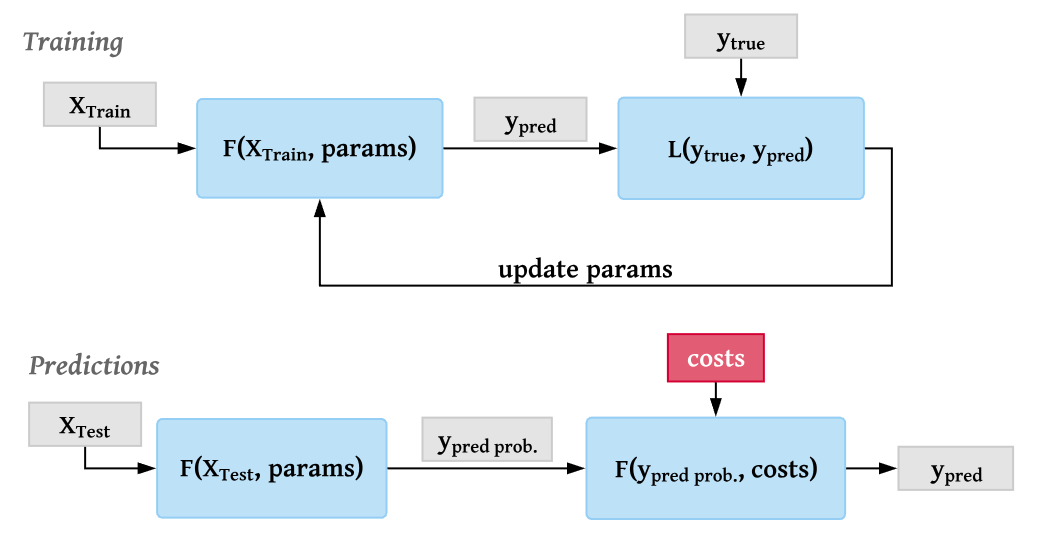
\includegraphics[width=\linewidth]{images/cost_sensitive_classification.png}
		\caption{Schemat przedstawiający proces uczenia klasyfikatora wrażliwego na koszt. Źródło: https://towardsdatascience.com/fraud-detection-with-cost-sensitive-machine-learning-24b8760d35d9}
		\label{cdc}
	\end{figure}
	\subsection{Optymalizacja progu}
		Metoda optymalizacji progu jest popularną metodą wyznaczania odpowiedniego progu prawdopodobieństwa powyżej którego wszystkie obserwacje oznaczamy jako pozytywnie zaklasyfikowane. Może być ona wykorzystywana nie tylko do problemów wrażliwych na koszt, lecz do dowolnie zdefiniowanego zagadnienia, w której wyznaczenie progu jest potrzebne. Jej sformułowanie wygląda następująco
		$$ \argmin_{th \in [0,1]} f(\ylab{y}{true}, \ylab{y}{decision}) \text{,} $$
		gdzie 
		\begin{itemize}
			\item $ f(\dot) $ - miara skuteczność modelu, np. skuteczność,
			\item $ \ylab{y}{true} = (c_i)_{i=1}^n $ - wektor prawdziwych oznaczeń ,
			\item $ \ylab{y}{decision} = (p_i > th)_{i=1}^n $ - wektor binarnych odpowiedzi modelu,
			\item $ p_i $ - przewidywana wartość prawdopodobieństwa dla i-tej obserwacji,
			\item $ \text{th} $ - wartość progu decyzyjnego.
		\end{itemize}{}
		W naszym przypadku funkcja $f$ to funkcja kosztu całkowitego (\ref{koszt-calkowity}). Innymi słowy, w tym przypadku będziemy szukać takiego progu decyzyjnego, który zminimalizuje sumaryczną wartość kosztów.
		
		% TODO: Opcjonalne - odwołać się do przypadków wielu minimum. Opisać algorytmiczne wyznaczanie tej wartości.
	\subsection{Minimalizacja ryzyka bayesowskiego}
	
	Metoda minimalizacji ryzyka bayesowskiego (\textit{ang. Bayesian Minimum Risk}) polega na przypisaniu odpowiedniej wartości reprezentującej ryzyko zaklasyfikowania danej obserwacji jako pozytywnej lub negatywnej, które definiujemy w następujący sposób:
	$$ R(p_1|x_i) = L(p_1|y_1)P(p_1|x_i) + L(p_1|y_0)P(y_0|x_i) \text{,}$$
	$$ R(p_0|x_i) = L(p_0|y_0)P(p_0|x_i) + L(p_0|y_1)P(y_1|x_i) \text{,}$$
	gdzie
	\begin{itemize}
		\item $P(p_1|x_i)$, $P(p_0|x_i)$ - oznacza estymowane przez model prawdopodobieństwo i oczywiście $P(p_0|x) = 1 - P(p_1|x)$,
		\item $L(p_{i}|y_{j})$ oraz $i,j \in \{l,f\}$ - funkcja kosztu,
		\item $x_i$ - i-ta obserwacja.
	\end{itemize}{}
	Klasyfikacja danej obserwacji jest opisana następującą nierównością:
	$$ R(p_1|x_i) \leq R(p_0|x_i)$$
	I oznacza ona, że klasyfikujemy dany przykład jako pozytywny, jeżeli ryzyko takiej decyzji jest mniejsze niż zaklasyfikowania danej obserwacji jako negatywną. 
	Po przeprowadzaniu odpowiednich przekształceń algebraicznych otrzymujemy następujący wzór na klasyfikację przykładu jako pozytywny:
	$$ P(p_1|x_i) \ge \frac{L(p_1|y_0) - L(p_0|y_0)}{L(p_0|y_1) - L(p_1|y_1) - L(p_0|y_0) + L(p_1|y_0)} \text{.}$$
	W przypadku gdy za funkcję kosztu przyjmiemy odpowiednie wartość z macierzy kosztu, to otrzymujemy następujący prób decyzyjny:
	$$ p \ge \frac{C_{FP_i} - C_{TN_i}}{C_{FN_i} - C_{TP_i} - C_{TN_i} + C_{FP_i}} \text{.}$$

\section{Cost Sensitive Training}
	Drugą podgrupą metod wrażliwych na koszt jest \textit{Cost Sensitive Trainig}. Są to metody, które już na etapie treningu modelu biorą pod uwagę koszt związany z klasyfikacją danej obserwacji. Schemat uczenia modelu jest przedstawiony na Rysunku \ref{cst}. Model jako wejście otrzymuje zbiór danych treningowych, następnie dokonuje predykcji i na bazie prawdziwych odpowiedzi oraz kosztów wyznaczana jest skuteczność modelu i kolejno aktualizowane są wagi, a cały proces jest iteracyjnie powtarzany aż do momentu osiągnięcia zadanego kryterium stopu.
	\begin{figure}
		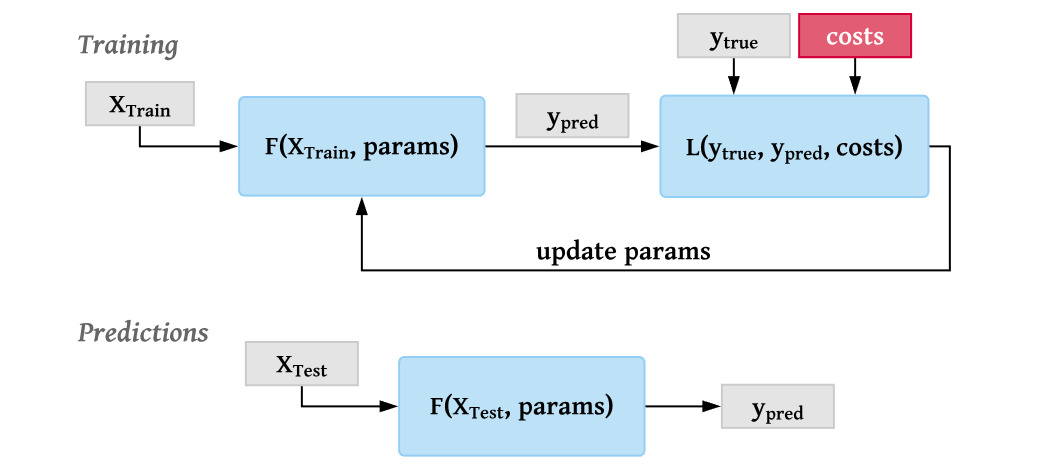
\includegraphics[width=\linewidth]{images/cost_sensitive_training.png}
		\caption{Schemat przedstawiający proces uczenia modelu wrażliwego na koszt. Źródło: https://towardsdatascience.com/fraud-detection-with-cost-sensitive-machine-learning-24b8760d35d9}
		\label{cst}
	\end{figure}	

\subsection{Regresja logistyczna wrażliwa na koszt}
		Pierwszy modelem, który stosunkowo łatwo przystosować do bycia wrażliwym na koszt jest regresja logistyczna. Kontynuując rozważania z podrozdziału \ref{reg-log} chcemy, aby funkcja straty przyjmowała następujące wartości, które odpowiadają wartościom z macierzy kosztu:
		$$
		J^c_i(\theta)=\left\{
		\begin{array}{rl}
		C_{TP_i}, &\mbox{if $y_i = 1$ and $\htx \approx 1$}, \\
		C_{TN_i}, &\mbox{if $y_i = 0$ and $\htx \approx 0$}, \\
		C_{FP_i}, &\mbox{if $y_i = 0$ and $\htx \approx 1$}, \\
		C_{FN_i}, &\mbox{if $y_i = 1$ and $\htx \approx 0$}.
		\end{array}
		\right.
		$$
		W rezultacie funkcją, która zachowuje się w powyższy sposób jest:
		\begin{talign*}
			J^c(\theta) &= \frac{1}{N} \sum_{i=1}^{N} \bigg( y_i \Big( \htx C_{TP_i} + (1 - \htx)C_{FN_i} \Big) \\
			&+ (1-y_i) \Big( \htx C_{FP_i} + (1 - \htx)C_{TN_i} \Big) \bigg)
		\end{talign*}
		
		\begin{figure}
			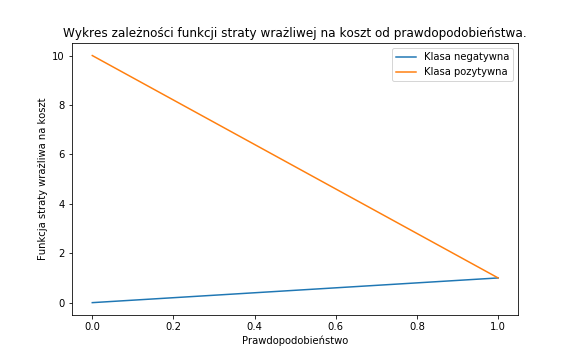
\includegraphics[width=\linewidth]{images/cost_sensitive_ce.png}
			\label{cost-sensitive-loss-function}
			\caption{Wykres zależności wrażliwej na koszt funkcji straty od prawdopodobieństwa predykcji danej obserwacji. Kolor niebieski przedstawia wykres dla próbki o prawdziwej klasie pozytywnej, natomiast kolor pomarańczowy dla negatywnej. Wykres dla przykładowych wartości: $C_{\text{TP}} = 1 \text{, } C_{\text{FN}} = 10 \text{, } C_{\text{FP}} = 1 \text{, } C_{\text{TN}} = 0$.}
		\end{figure}
	
		% TODO: Opisać wykres.
		Następnie standardowo wykorzystując algorytm optymalizujący, który znajdzie odpowiednie współczynniki modelu trenujemy model predykcyjny.
\subsection{Drzewo decyzyjne wrażliwe na koszt}
	Analogicznie jak w przypadku regresji logistycznej w celu wprowadzenia kosztu do treningu drzewa decyzyjnego musimy uzależnić proces powstawania modelu od kosztu danej próbki. Naturalnym miejscem dla drzewa decyzyjnego jest proces podziału danego węzła na kolejne węzły bądź liście. Dlatego definiujemy następującą miarę zanieczyszczenia, która następujący wzór:
	$$ I_c(\es) = min \left\{ Cost(f_0(\es)), Cost(f_1(\es)) \right\} \text{.}$$
	Dodatkowo w przy dokonywaniu predykcji klasyfikacja na wartość pozytywną bądź negatywną następuje wg następującego kryterium:
	$$ f(\es) =  \left\{
		\begin{array}{rl}
			0, &\mbox{jeżeli $\text{Cost}(f_0(\es)) \leq \text{Cost}(f_1(\es))$}, \\
			1, &\mbox{w przeciwnym wypadku},
		\end{array}{}
	\right.
	$$
	gdzie jak zawsze 1 oznacza wartość pozytywną, a 0 negatywną. 
	Z poprzednich rozważań oczywiście możliwe jest stworzenie modeli typu \textit{ensemble}, w których klasyfikatorem bazowym byłoby drzewo decyzyjne wrażliwe na koszt, natomiast jest to poza obszarem badań aktualnej pracy.
	
\section{Miary skuteczności modeli}
	
	Opis miar...
	
	\subsection{Macierz pomyłek}
	
	Jedną z najpopularniejszych metod wykorzystywanych do oceny skuteczności modeli w zadaniach klasyfikacji binarnej jest macierz pomyłek. Oznaczone dane zestawiamy z klasami nadanymi przez model, a następnie sprawdzamy czy poprawnie zaklasyfikowaliśmy poszczególne obserwacje. W ten sposób powstają cztery możliwe sytuacje, które są przedstawione w Tabeli \ref{macierz-pomylek}: 
	\begin{itemize}
		\item Prawdziwie pozytywna klasyfikacja (\textit{ang. True Positive (TP)}) - obserwacja była pozytywna i zaklasyfikowaliśmy ją jako pozytywną
		\item Fałszywie negatywna klasyfikacja (\textit{ang. False Negative (FN)}) - obserwacja była pozytywna i zaklasyfikowaliśmy ją jako negatywną. W nomenklaturze statystycznej nazywana również błędem drugiego rodzaju.
		\item Fałszywie pozytywna klasyfikacja (\textit{ang. False Positive (FP)}) - obserwacja była negatywna i zaklasyfikowaliśmy ją jako pozytywną. W nomenklaturze statystycznej nazywana również błędem pierwszego rodzaju.
		\item Fałszywie negatywna klasyfikacja (\textit{ang. False Positive (FN)}) - obserwacja była pozytywna i zaklasyfikowaliśmy ją jako negatywną
	\end{itemize}
	\begin{table}[h]
		\begin{center}
			\makegapedcells
			\begin{tabular}{cc|cc}
				\multicolumn{2}{c}{}     &   \multicolumn{2}{c}{Predykcja} \\
				&            &   Pozytywna &   Negatywna     \\ 
				\cline{2-4}
				\multirow{2}{*}{\rotatebox[origin=c]{90}{Prawda}} & Pozytywna   & TP         & FN              \\
				& Negatywna   & FP         & TN              \\ 
				\cline{2-4}
			\end{tabular}
		\end{center}
		\caption{Macierz pomyłek}
		\label{macierz-pomylek}
	\end{table}
	
	Dodatkowo na podstawie macierzy pomyłek możemy zdefiniować następujące miary skuteczności modeli:
	
	Skuteczność, która określa jaki procent wszystkich obserwacji zaklasyfikowaliśmy poprawnie.
	$$ \text{Skuteczność} = \frac{TP + TN}{TP + FP + FN + TN} $$
	Precyzja, która mierzy ile procent zaklasyfikowanych próbek jako pozytywne faktycznie były pozytywne.
	$$ \text{Precyzja} = \frac{TP}{TP + FP} $$
	Czułość, która mówi Nam o procencie znalezionych wszystkich pozytywnych przypadków.
	$$ \text{Czułość}= \frac{TP}{TP + FN} $$
	F1 Score, który jest średnią harmoniczną precyzji oraz czułości.
	$$ \text{F1 Score} = 2 \cdot \frac{\text{Precyzja} \cdot \text{Czułość}}{\text{Precyzja} + \text{Czułość}} $$
	Wszystkie wyżej wspomniane miary skuteczności przyjmują wartości z zakresu $[0,1]$ oraz wyższa wartość oznacza lepszy model.
	
	
	\subsection{Miary skuteczności modeli wrażliwe na koszt}
	
	Motywacją do powstania miar wrażliwych na koszt jest rzeczywista ewaluacja modeli. Podstawowe metryki nie uwzględniają różnicy w kosztach pomyłki dla FP i FN. Ponadto koszt fraudów znacząco różni się w zależności od przypadku.
	
	W celu wprowadzenia potrzebnych miar skuteczności potrzebujemy wprowadzić tzw. macierz kosztu, która jest zaprezentowana w Tabeli \ref{macierz-kosztu}, gdzie poszczególne komórki oznacza odpowiadające wartość kosztu predykcji. 
	\begin{table}[h]
		\begin{center}
			\makegapedcells
			\begin{tabular}{cc|cc}
				\multicolumn{2}{c}{}     &   \multicolumn{2}{c}{Predykcja} \\
				&            &   Oszustwo &   Normalna     \\ 
				\cline{2-4}
				\multirow{2}{*}{\rotatebox[origin=c]{90}{Prawda}} & Oszustwo   & $C_{TP_{i}}$         & $C_{FN_{i}}$              \\
				& Normalna   & $C_{FP_{i}}$         & $C_{TN_{i}}$              \\ 
				\cline{2-4}
			\end{tabular}
		\end{center}
		\caption{Macierz kosztu}
		\label{macierz-kosztu}
	\end{table}
	Następnie definiujemy następującą wartość:
	$$ \text{Koszt}(f(\iks_{i}^{*})) = y_i (c_i C_{TP_i} + (1-c_i)C_{FN_i}) + (1-y_i)(c_i C_{FP_i} + (1-c_i)C_{TN_i}) \text{,}$$
	gdzie 
	\begin{itemize}
		\item $\iks_{i}^{*} = [\iks_i, C_{TP_{i}}, C_{FP_{i}}, C_{FN_{i}}, C_{TN_{i}}]$ - wektor zawierający wartości cech i-tej obserwacji rozszerzony o koszt klasyfikacji
		\item $C_{\cdot}$ - koszt klasyfikacji i-tej obserwacji
		\item $f(\cdot)$ - model predykcyjny
		\item $y_i$ - prawdziwa wartość i-tej obserwacji
		\item $c_i$ - predykcja dla i-tej obserwacji
	\end{itemize}{}
	Następnie wprowadzamy następujące miary skuteczności modeli:
	\begin{equation}
	\label{koszt-calkowity}
	\text{Koszt całkowity}(f(\boldsymbol{S})) = \sum_{i=1}^{N}\text{Cost}(f(\boldsymbol{x}_{i}^{*}))
	\end{equation} 
	\begin{equation}
	\text{Oszczędności} = \frac{\text{Koszt}_{l}(\bes) - \text{Koszt}(f(\bes))}{\text{Koszt}_{l}(\bes)}
	\end{equation}
	gdzie
	\begin{itemize}
		\item $ \bes $ - data set
		\item $ \text{Koszt}_0 = min\{\text{Cost}(f_{0}(\bes), \text{Koszt}(f_{1}(\bes)\} $
		\item $ f_{a}(\bes) = \boldsymbol{a} $ gdzie $a \in \{0,1\}$
	\end{itemize}{}
	Wartość $ f_{a}(\bes)$ możemy rozumieć jako przypadek naiwnego modelu, który wszystkim obserwacjom przyznaje wartość $a$. Natomiast $ \text{Koszt}_0 $ oznacza wybranie naiwnego klasyfikatora, który generuje mniejsze koszty. Zatem ostatecznie Oszczędności możemy rozumieć jako procentową wartość o ile testowany model jest lepszy od naiwnego klasyfikatora.
	
	% TODO: Analiza wartości minimalnych oraz maksymalnych Kosztu całkowitego oraz Oszczędności. 
	
\chapter{Eksperyment}
	W celu porównania skuteczności metod wrażliwych na koszt względem siebie wykonamy eksperyment, którego celem będzie sprawdzenie, który z modeli lub ich kombinacja przyniesie największe oszczędności na zbiorze danych dot. oszustw z wykorzystaniem kart kredytowych. Jako dodatkowy wskaźnik wykorzystamy miarę skuteczności modelu F1 Score, która będzie w stanie odpowiedzieć jak zmieniła się ogólna skuteczność modelu.

\section{Dane}
	Do eksperymentu zostanie wykorzystany zbiór danych Credit Card Fraud Detection zawierający 284,807 transakcji w tym zaledwie 492 oszustw. Tabela składa się z 30 kolumn, w tym 28 z nich są to zanonimizowane zmienne numeryczne, które były wcześniej poddane transformacji PCA (\textit{ang. Principal Component Analysis}), a dodatkowo posiadamy informacje dot. czasu transakcji oraz kwoty. Ponadto wśród danych nie ma brakujących wartości. Podczas modelowania pominiemy zmienną czasową, ponieważ sama w sobie nie zawiera ona istotnej informacji, natomiast stworzenie znaczących zmiennych nie jest istotą przeprowadzanego eksperymentu. 
	
	Mimo tego, że dane zostały poddane anonimizacji, to na podstawie \ref{} możemy domyślać się z jakimi zmiennymi mieliśmy do czynienia przed transformacjami. Podczas procesu dokonywania transakcji standardowo zbierane są: ID klienta, data dokonania transakcji, kwota, lokalizacja, typ transakcji (przykładowo płatność internetowa, płatność stacjonarna, wypłata z bankomatu), beneficjent transakcji (przykładowo linie lotnicze, hotel, wypożyczalnia samochodów itp.), historyczna informacja dot. czy dana transakcja była oszustwem, wiek klienta, kraj zamieszkania, kod pocztowy, typ karty (przykładowo VISA, MasterCard itp.). Na podstawie wymienionych informacji tworzy się agregaty czasowe bazujące na historii, które składają się z następujących kombinacji zmiennych:
	\begin{itemize}
		\item Klient, karta kredytowa;
		\item Typ transakcji, beneficjent transakcji, kategoria beneficjenta, kraj;
		\item W ciągu ostatnich godzin/dni/tygodni/miesięcy;
		\item Ilość, średnia lub suma transakcji.
	\end{itemize}
	Przykładowymi zmiennymi, które powstają w tym procesie są: Ilość transakcji dla tego samego klienta w ciągu ostatnich 6/12/24 godzin, Średnia wartość transakcji dla danego klienta z ostatniego tygodnia. 
	
	Informacja, która jest najbardziej istotna z punktu widzenia naszego modelowania, to rozkład oraz charakterystyka zmiennej dot. kwoty transakcji. Na Rysunku \ref{} znajduje się wykres rozkładu ... 
	
	Warto zauważyć, że najpopularniejszymi wartościami transakcji są: 
	
	Na podstawie przeprowadzonej analizy definiujemy w Tabeli \ref{macierz-kosztu-eksperyment} macierz kosztu dla tego eksperymentu, gdzie $C_a$ to koszt administracyjny podjęcia sprawy przez analityka, który sprawdza czy dana obserwacja jest faktycznie oszustwem niezależnie od tego jaki był jego ostateczny werdykt, $\text{Amt}_i$ to wartość transakcji jaką utracimy w przypadku nie wskazanie danej obserwacji jako oszustwa, natomiast zerowa wartość kosztu dla normalnej transakcji, która była prawidłowo wskazana, wynika z braku konieczności podjęcia inwestygacji oraz strat z tego wynikających.
	
	\begin{table}[h]
		\begin{center}
			\makegapedcells
			\begin{tabular}{cc|cc}
				\multicolumn{2}{c}{}     &   \multicolumn{2}{c}{Predykcja} \\
				&            &   Oszustwo &   Normalna     \\ 
				\cline{2-4}
				\multirow{2}{*}{\rotatebox[origin=c]{90}{Prawda}} & Oszustwo   & $C_a$         & $\text{Amt}_i$              \\
				& Normalna   & $C_a$         & $0$              \\ 
				\cline{2-4}
			\end{tabular}
		\end{center}
		\caption{Macierz kosztu dla eksperymentu.}
		\label{macierz-kosztu-eksperyment}
	\end{table}
	
\section{Opis eksperymentu}
	Eksperyment został przeprowadzony w następujący sposób:
	50-krotnie dzielimy zbiór danych w proporcjach 50:17:33 na zbiór treningowy, walidacyjny oraz testowy. Następnie uczymy wszystkie modele na zbiorze treningowym. Dla modelu XGBoost wykorzystujemy zbiór walidacyjny do procesu wczesnego zatrzymywania (\textit{ang. Early stopping}), natomiast dla modeli BMR oraz TO korzystamy z tego zbioru jako zbiór treningowy. Następnie dla wszystkich modeli dokonujemy predykcyji na zbiorze testowym i mierzymy skuteczność typowań. Warto wspomnieć, że 50-krotne losowanie nowych podziałów zbioru ma na celu zmiejszenie ryzyka, że wynik zależy od wylosowanej próbki. Ponadto wykorzystano tą technikę w opozycji do standardowej warstwowej walidacji krzyżowej (\textit{ang. Stratified Cross Validation}) z uwagi na chęć uniknięcia zbyt małej próbki testowej w przypadku walidacji krzyżowej z dużą ilością podziałów. Następnie dla każdego modelu została obliczona wartość średnia oraz odchylenie standardowe dla wcześniej określonych miar.
	
	Do implementacji skryptów został wykorzystany język programowania Python wraz z bibliotekami costcla, sklearn, pandas, numpy, matplotlib oraz język programowania bash.

\section{Wyniki}
	Lorem ipsum ...
	
	\begin{figure}[h]
		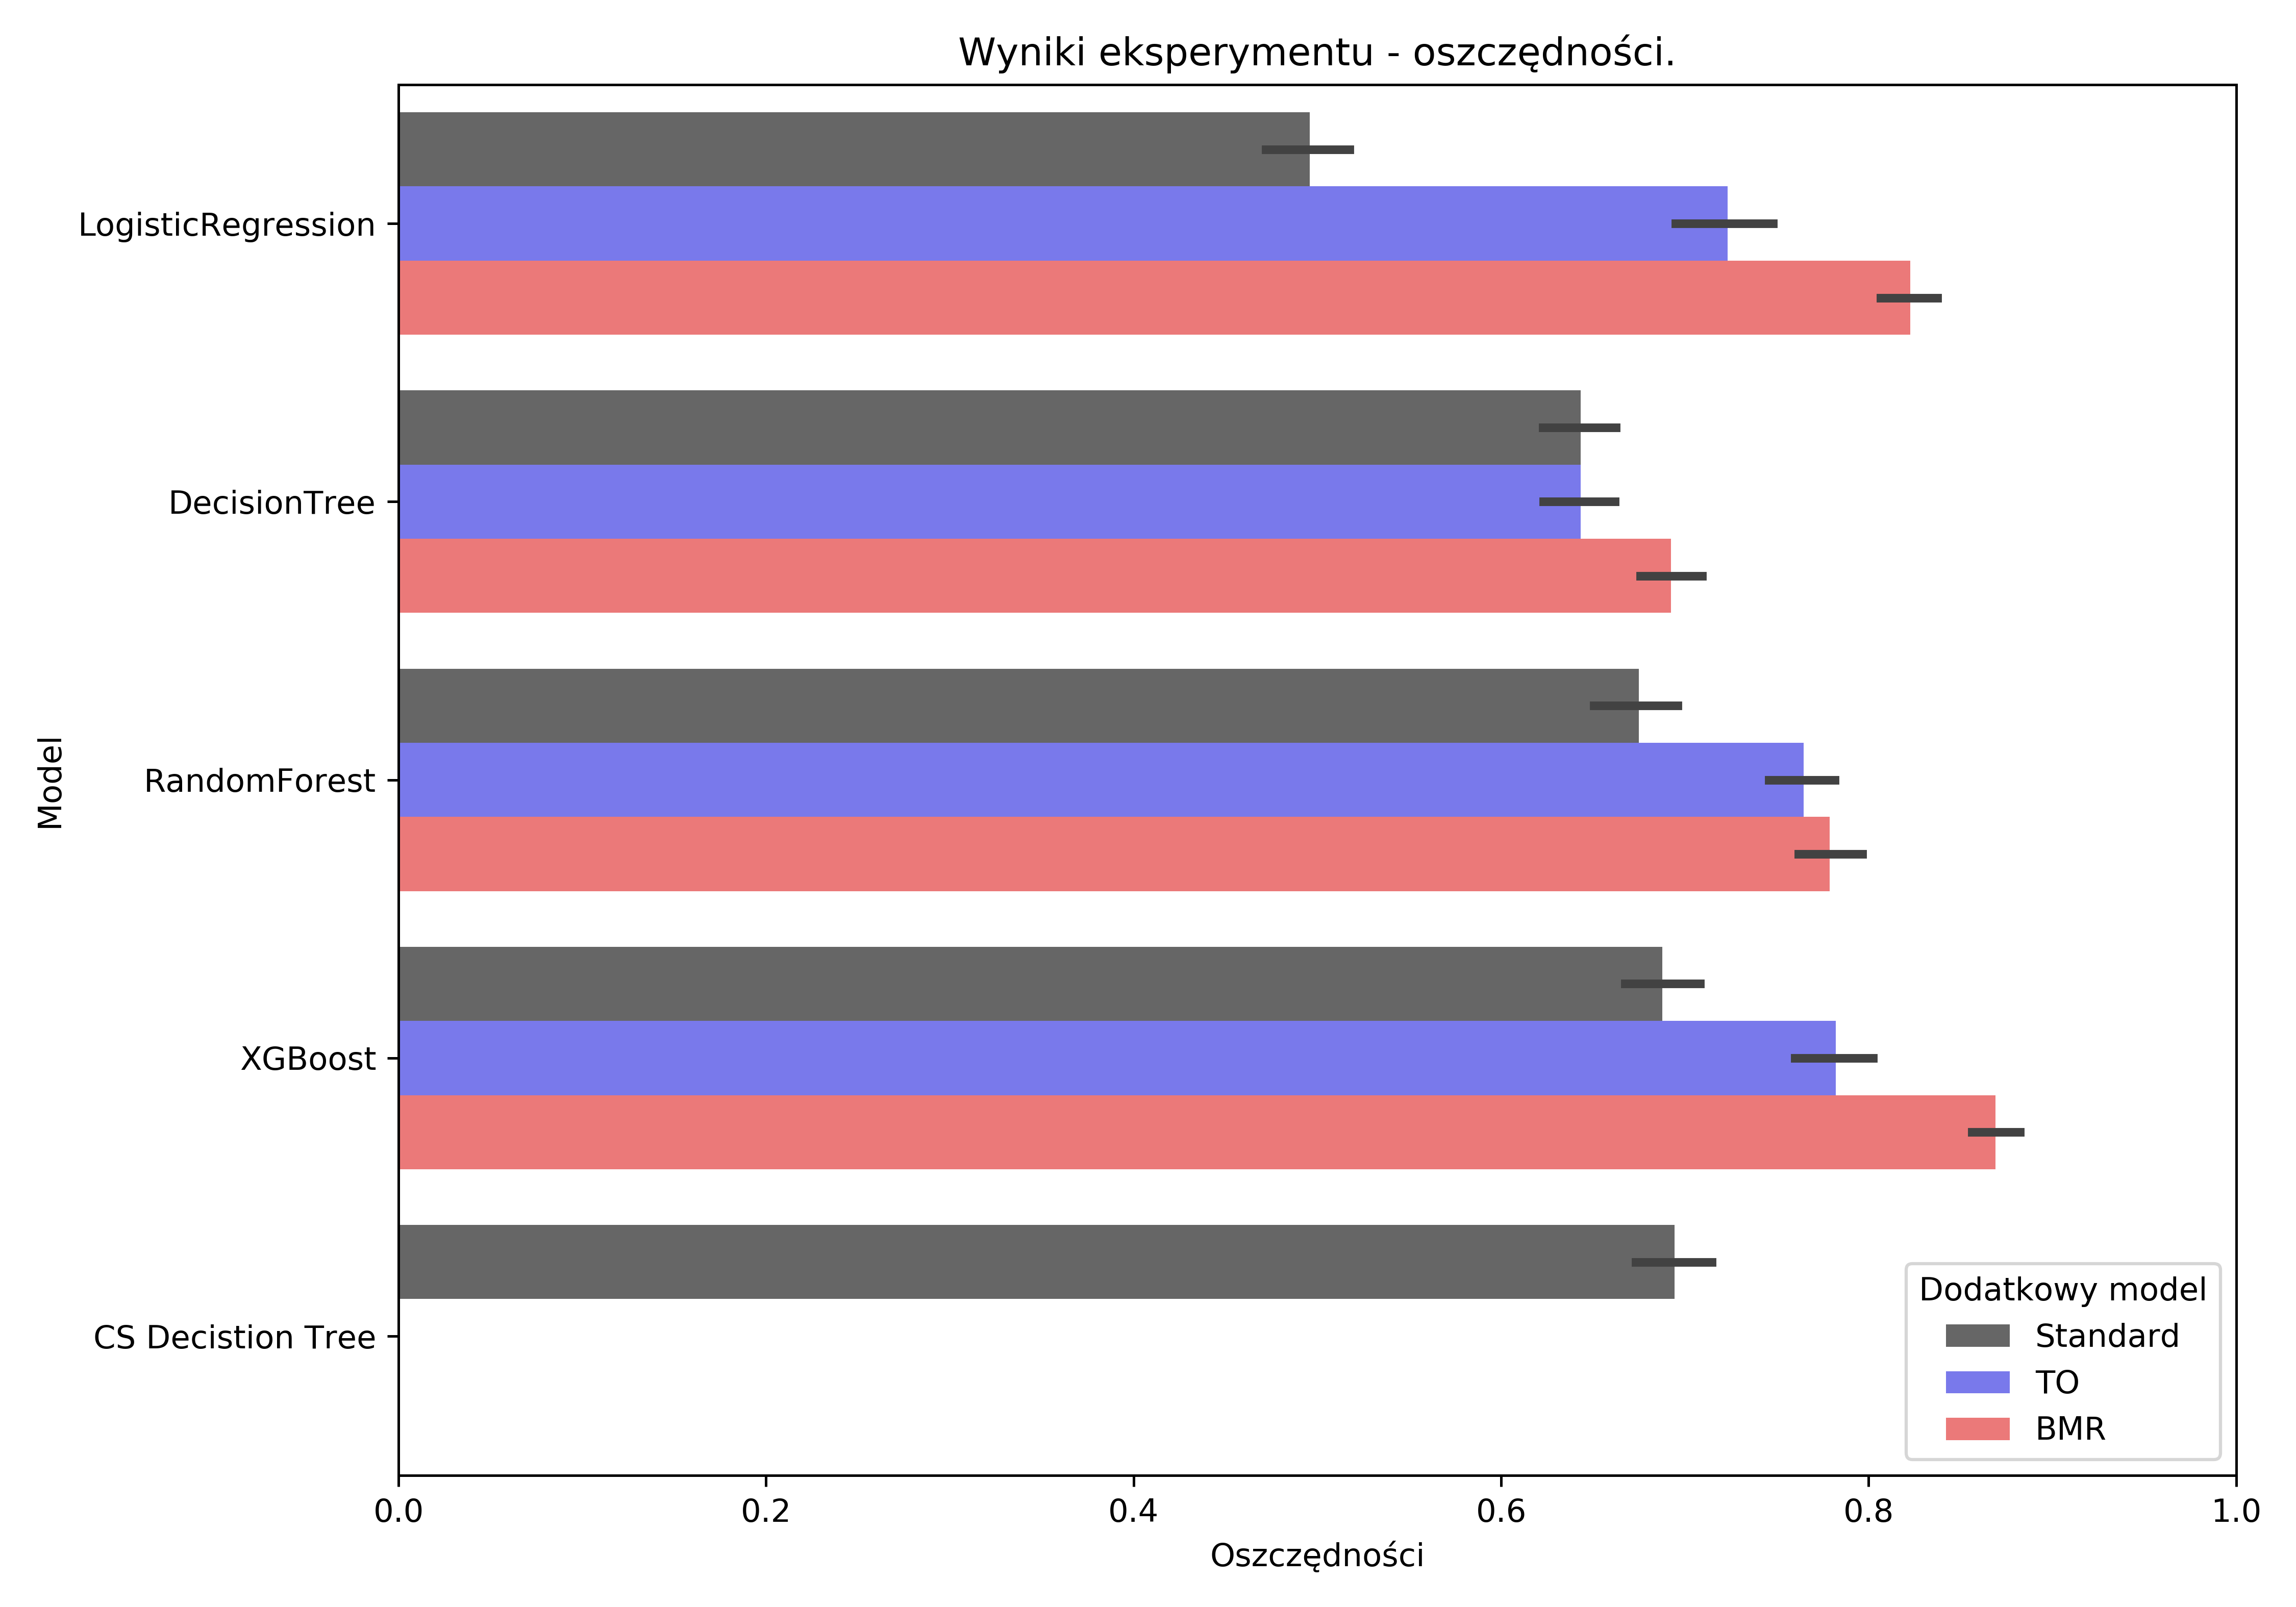
\includegraphics[width=\linewidth]{images/100_config1-Savings.png}
		\label{results-savings}
		\caption{Wyniki eksperymentu dla miary skuteczności Oszczędności.}	
	\end{figure}
	% TODO: Caption
	
	\begin{figure}[h]
		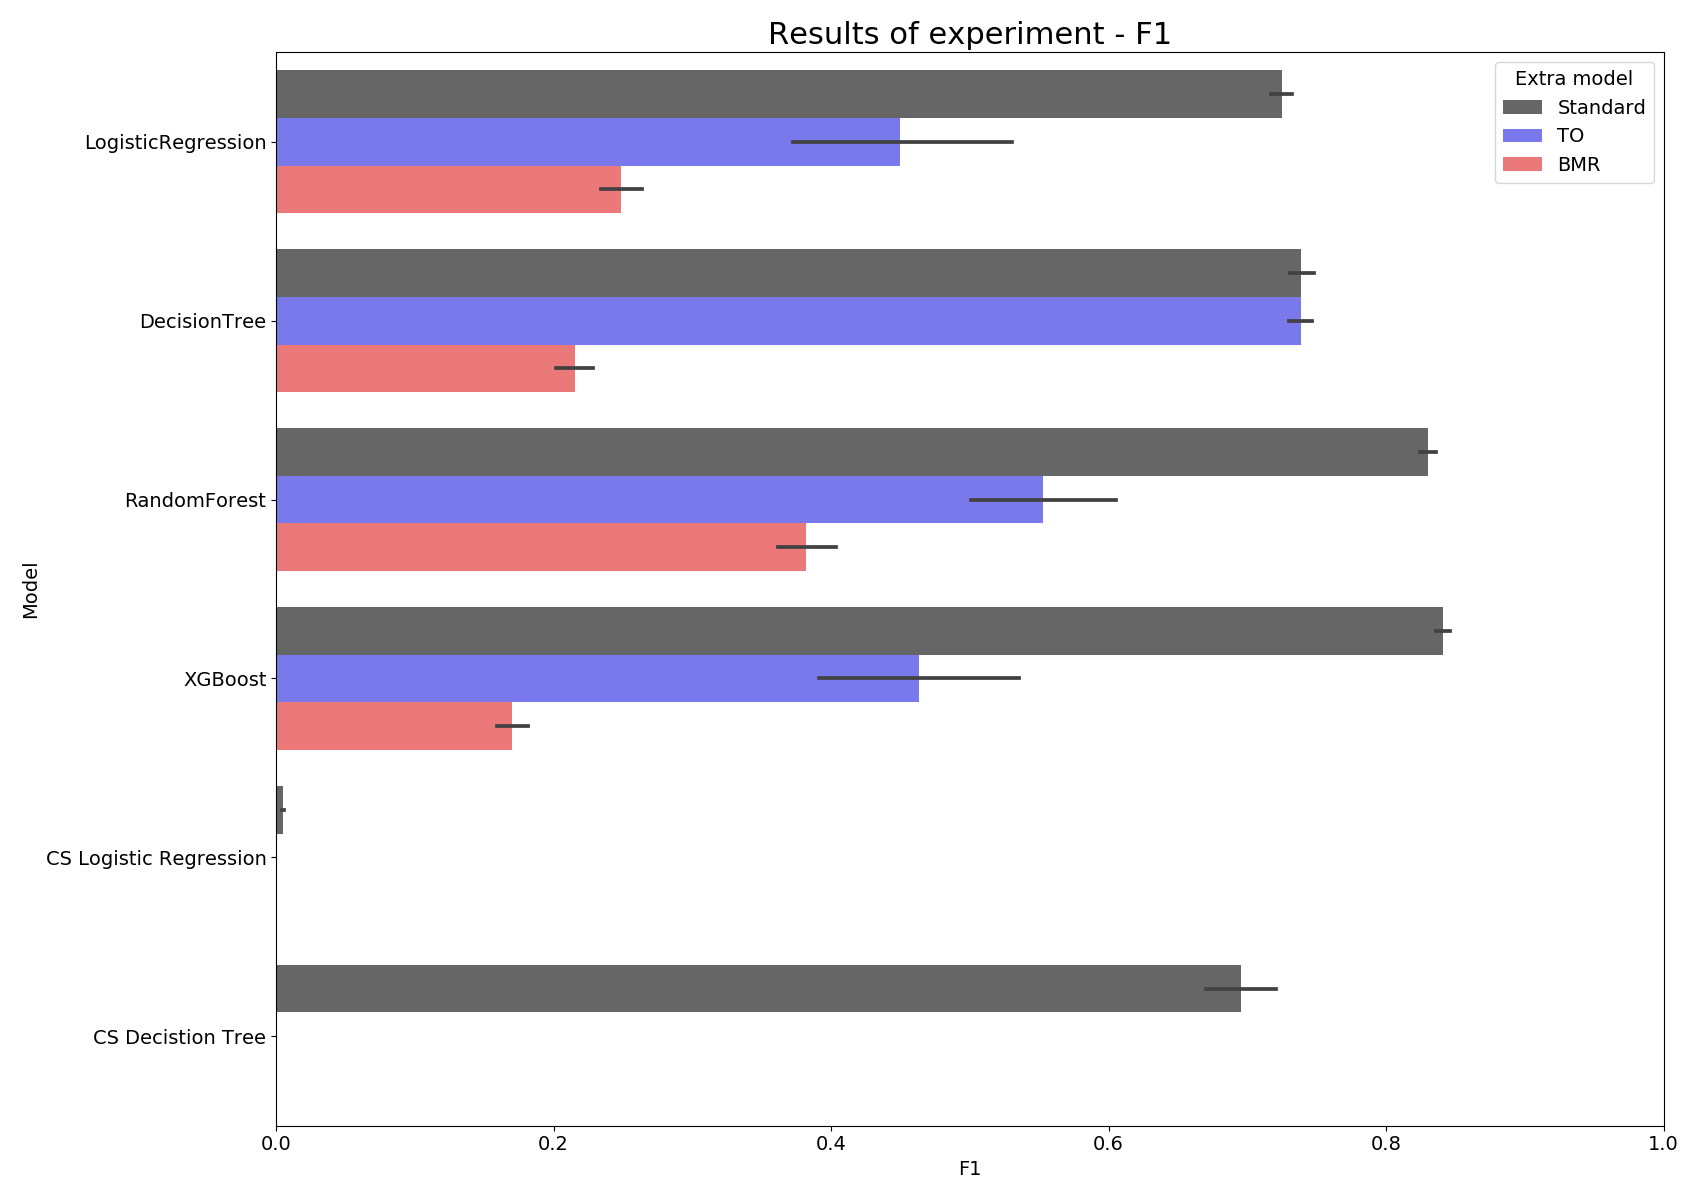
\includegraphics[width=\linewidth]{images/100_config1-F1.png}
		\label{results-f1}
		\caption{Wyniki eksperymentu dla miary skuteczności F1-Score.}
	\end{figure}
	% TODO: Caption	
	
	Korzystając z Rysunku \ref{results-savings} możemy zauważyć, że: ...
	
	Korzystając z Rysunku \ref{results-f1} możemy zauważyć, że: ...	
	
	% TODO: Testy statystyczne

\chapter{Podsumowanie}


% Bibliografia
\nocite{*}

\bibliographystyle{plain}
\bibliography{references}

\end{document}

% Referencje
% https://www.youtube.com/watch?v=YCNkxaVDiA0

% TODO:
% Resampling to LR
% Streszczenie
